\documentclass{beamer}

\mode<presentation> {
\usetheme{Madrid}
}

\usepackage{graphicx}
\usepackage{booktabs}
\usepackage{polski}
\usepackage[polish]{babel}
\usepackage[utf8]{inputenc}
\usepackage[T1]{fontenc}
\usepackage[utf8]{luainputenc}
\usepackage{pgfgantt}
\usepackage{caption}
\usepackage{mwe}

% Strona tytułowa
\usepackage{pgfplots}
\usepackage{siunitx}
\usepackage{paracol}
\usepackage{gensymb}

% Pływające obrazki
\usepackage{float}
\usepackage{svg}
\usepackage{graphicx}
\usepackage{subfig}


\sisetup{group-digits=true,
        %  group-four-digits=true,
        round-precision=4,
        group-separator={},
        output-decimal-marker={,}}

\DeclareCaptionFormat{citation}{%
   \ifx\captioncitation\relax\relax\else
     \captioncitation\par
   \fi
   #1#2#3\par}
\newcommand*\setcaptioncitation[1]{\def\captioncitation{\tiny{\textit{Źródło:}~#1}\medskip}\normalsize}
\let\captioncitation\relax
\captionsetup{format=citation,justification=centering}

\usetikzlibrary{pgfplots.groupplots}
\sisetup{detect-weight,exponent-product=\cdot,output-decimal-marker={,},per-mode=symbol,binary-units=true,range-phrase={-},range-units=single}

%wymiar tekstu
\def\figurename{Rys.}
\def\tablename{Tab.}

%----------------------------------------------------------------------------------------
%	TITLE PAGE
%----------------------------------------------------------------------------------------

\title[WEDT - Projekt]{Wprowadzenie do eksploracji danych tekstowych w~sieci~WWW}

\author[Konieczka, Poturała, Sikora]{Maria Konieczka \and Alicja Poturała \and Jakub Sikora} 

\date{3 czerwca 2020}
\institute[]{Odpowiadanie na pytania ogólne zadane w~języku polskim}

\AtBeginSection[]
{
    \begin{frame}[plain, noframenumbering]
        \frametitle{Agenda}
        \tableofcontents[currentsection]
    \end{frame}
}

\begin{document}

\begin{frame}
\titlepage
\end{frame}

\begin{frame}
  \frametitle{Agenda}
  \tableofcontents
\end{frame}

\section{Wprowadzenie w problem}

\begin{frame}
  \frametitle{Odpowiadanie na pytania}

\end{frame}

\begin{frame}
  \frametitle{Założenia systemu}

\end{frame}

\section{Algorytm wyszukiwania odpowiedzi}
\begin{frame}
  \frametitle{Ogólny opis algorytmu wyszukiwania}
  \bigskip
  \begin{figure}
    \centering
    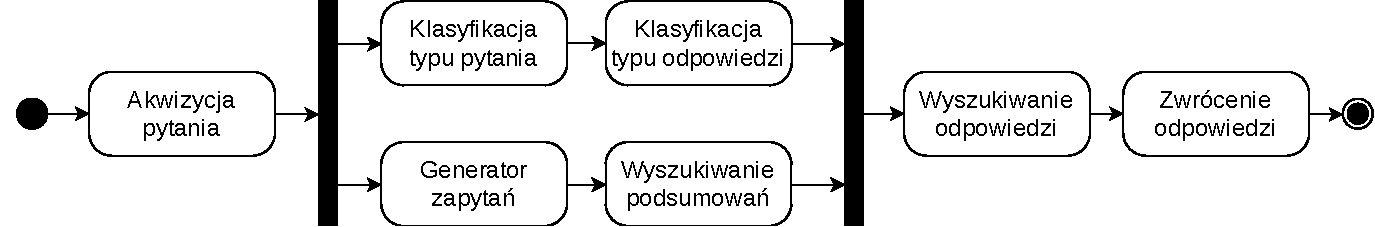
\includegraphics[width=\columnwidth]{figures/WEDT-Algorytm-Rotated.pdf}
    \caption{Ogólny schemat blokowy algorytmu wyszukiwania odpowiedzi}
    \label{fig:ir-algorytm}
  \end{figure}
\end{frame}

\begin{frame}
  \frametitle{Akwizycja pytania}

\end{frame}

\begin{frame}
  \frametitle{Generacja zapytań}

\end{frame}

\begin{frame}
  \frametitle{Wyszukiwanie podsumowań}

\end{frame}

\begin{frame}
  \frametitle{Klasyfikacja typu pytania}

\end{frame}

\begin{frame}
  \frametitle{Klasyfikacja typu odpowiedzi}

\end{frame}

\begin{frame}
  \frametitle{Wyszukiwanie odpowiedzi}

\end{frame}

\begin{frame}
  \frametitle{Zwrócenie odpowiedzi}

\end{frame}

\section{Implementacja i korzystanie z systemu}
\begin{frame}
  \frametitle{Architektura mikroserwisowa}
  \begin{figure}
    \centering
    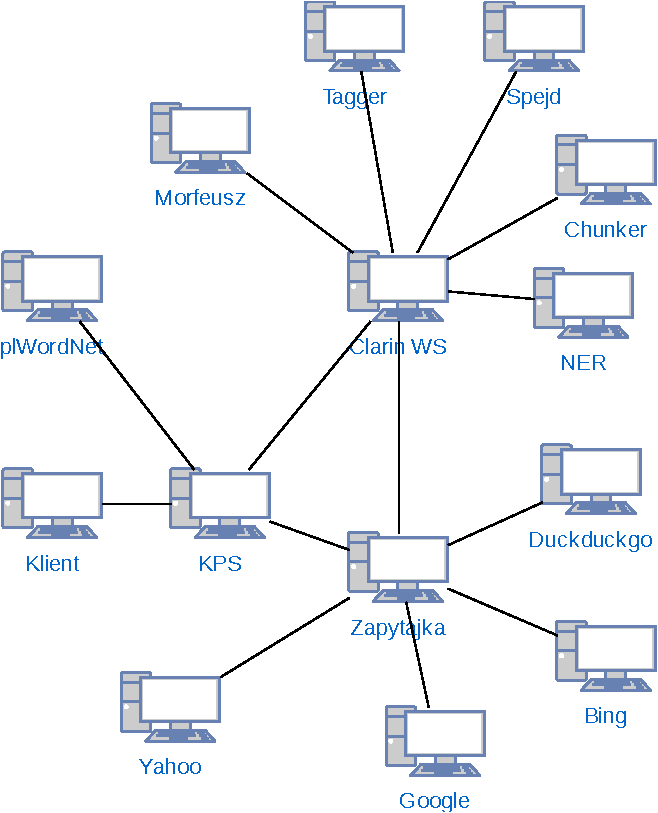
\includegraphics[width=0.5\columnwidth]{figures/WEDT-Uslugi.pdf}
    \label{fig:klient}
  \end{figure}
\end{frame}

\begin{frame}
  \frametitle{Implementacja systemu}
  \begin{block}{Implementacja modułów:}
    \begin{itemize}
      \item odpowiadania na pytania,
      \item klienta internetowego,
      \item \textit{webscrapera} wyszukiwarek internetowych.
    \end{itemize}
  \end{block}

  \begin{block}{Integracja z usługami:}
    \begin{itemize}
      \item plWordNet,
      \item CLARIN WS
      \begin{itemize}
        \item morfeusz,
        \item tagger,
        \item spejd,
        \item chunker,
        \item Named-Entity Recognition.
      \end{itemize}
    \end{itemize}
  \end{block}
\end{frame}

\begin{frame}
  \frametitle{Klient systemu} 
  \begin{figure}
    \centering
    \fbox{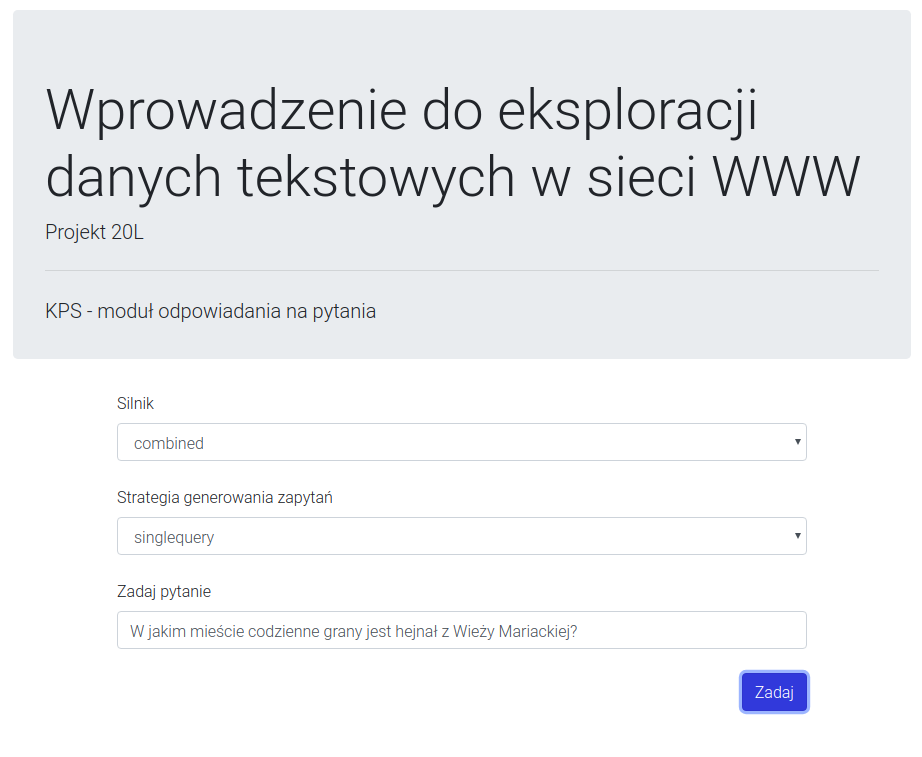
\includegraphics[width=0.7\columnwidth]{figures/kps.png}}
    \label{fig:klient}
  \end{figure}
\end{frame}

\begin{frame}
  \frametitle{Klient systemu} 
  \begin{figure}
    \centering
    \fbox{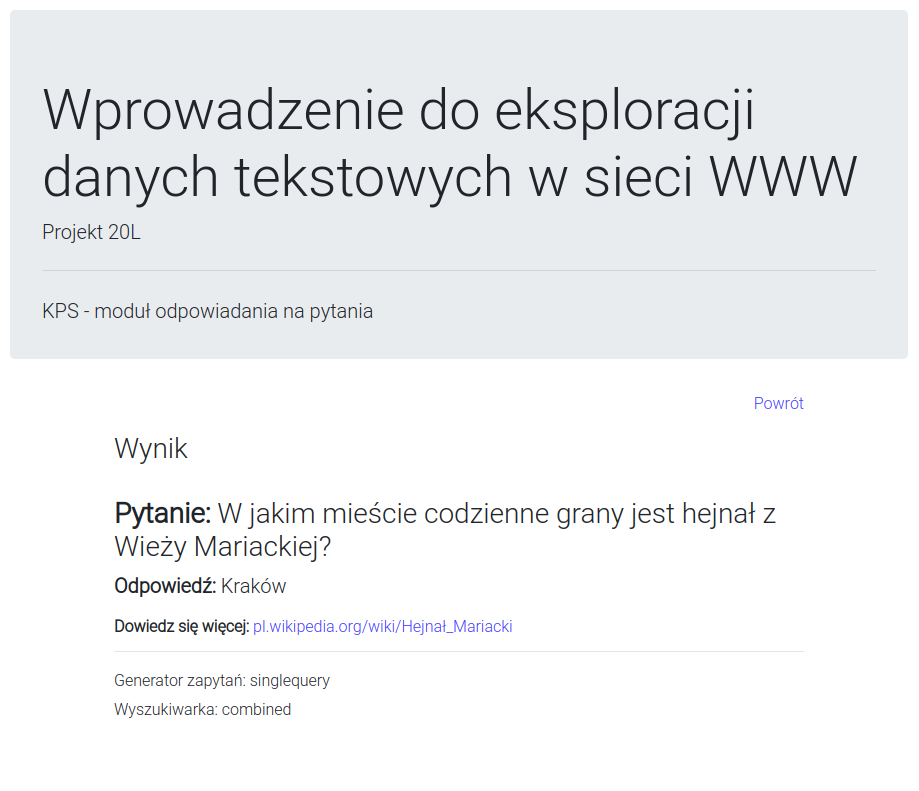
\includegraphics[width=0.7\columnwidth]{figures/kps-answer.png}}
    \label{fig:klient-odp}
  \end{figure}
\end{frame}

\section{Wyniki badań}
\begin{frame}
  \frametitle{Badanie wyszukiwarek internetowych}

\end{frame}

\begin{frame}
  \frametitle{Badanie strategii generacji zapytań}

\end{frame}

\section{Wnioski i przemyślenia}
\begin{frame}
  \frametitle{Wnioski z projektu}

\end{frame}

\begin{frame}
  \frametitle{Przemyślenia dotyczące zadania odpowiadania}

\end{frame}

\end{document}
